\section{L'entrée : le langage de \touist}
\subsection{Aperçu de l'expressivité de \touist\label{sec:sat_tobedone}}

\paragraph{Ensembles de domaines}
Avec le temps, nous avons remarqué que nous avions souvent besoin d'écrire des choses comme :
$$\begin{aligned}\bigwedge_{i \in \{1..9\}} \bigwedge_{j \in \{1..9\}}\bigwedge_{ m\in \{A,B,C,D,E,F,G,H,I\}} \hspace{2cm}\\ \left( P_{i,j,m}\IMPL \bigwedge_{n \in \{A,B,C,D,E,F,G,H,I\}|m\neq n}\NOT P_{i,j,n}\right)\end{aligned}$$
Si on lit $P_{i,j,m}$ comme  ``il y a la lettre $m$ dans la case $(i,j)$'' d'une grille $9\times 9$, la formule ci-dessus exprime qu'il y a \emph{au plus} une lettre parmi `A' ... `I' dans chaque case.

Ces ensembles $\{1..9\}$ et $\{A,B,C,D,E,F,G,H,I\}$ sont des \emph{ensembles de domaines}, et avec \touist\ l'utilisateur peut définir autant d'ensembles de domaines qu'il le souhaite, par exemple :

\begin{verbatim}
  $N=[1..9]
  $L=[A,B,C,D,E,F,G,H,I]
\end{verbatim}

et ainsi écrire la formule précédente comme :
$$\bigwedge_{i \in N} \bigwedge_{j \in N}\bigwedge_{ m\in L}P_{i,j,m}\IMPL \bigwedge_{n \in L|m\neq n}\NOT P_{i,j,n}$$
De plus, les opérations usuelles sur les ensembles ($\cup$, $\cap$, $\setminus$, \ldots) peuvent être utilisées pour définir d'autres ensembles.


\paragraph{Formules propositionnelles}

Les formules de \touist\ sont basées sur des variables propositionnelles (qui peuvent être indicées) et les opérateurs logiques usuels ($\AND$, $\OR$, $\IMPL$, $\NOT$, $\IFF$). Ainsi on peut taper des formules usuelles simples comme $Pluie \IMPL Nuages$. Mais en plus, nous fournissons des opérateurs logiques de haut niveau qui permettent d'exprimer des assertions complexes dans une forme très compacte.

\paragraph{Conjonctions et disjonctions généralisées}
Elles permettent d'exprimer des conjonctions et des disjonctions sur des formules contenant des paramètres qui varient, par exemple :
\begin{itemize}
\item $ \bigwedge_{i \in N} P_i$, où $N$ est l'ensemble de domaine défini précédemment.\\
  Elle représente la conjonction
  $P_1 \AND P_2 \AND \ldots \AND P_9$. 
\item $\bigvee_{i \in E} P_i$.
\end{itemize}

Bien s\^ur, ces opérateurs peuvent être imbriqués comme dans :
$$\bigwedge_{i \in N} \bigwedge_{j \in N}\bigvee_{ m\in L}P_{i,j,m}$$

qui indique que dans chaque cellule se trouve au moins une lettre.


\paragraph{Contraintes de cardinalité}
Il s'agissait de l'un des sujets "laissé pour le futur" de \cite{GaScSt2011}.
Ces opérateurs logiques moins classiques sont disponibles dans \touist\ : il permettent de réduire drastiquement la taille de certaines formules, ce sont : $\atM{}{}$, $\atL{}{}$ et $\exact{}{}$.\\ L'exemple suivant décrit leur signification :
\begin{itemize}
\item $\atM{i \in N}{2} P_i$ représente ``pour au plus deux valeurs de $i \in N$ $P(i)$ est vraie'';
\item $\atL{i \in N}{2} P_i$ représente ``pour au moins deux valeurs de $i \in N$ $P(i)$ est vraie'';
\item $\exact{i \in N}{2} P_i$ représente ``pour exactement deux valeurs de $i \in N$ $P(i)$ est vraie''.
\end{itemize}
La disjonction généralisée est en fait un cas particulier de ceci (au moins une est vraie), la conjonction aussi (au plus 0 est fausse), et le ou exclusif peut être vu comme exactement une parmi deux est vraie. \\
Rappelons qu'avec des opérateurs logiques classiques et avec $N$ contenant 9 éléments, $\atM{i \in N}{3} P_i$ devrait nécessiter une formule contenant 84 propositions $P_i$ puisque cela revient à choisir 3 parmi 9 ce qui donne $\binom{9}{3}$ possibilités, et ni $\bigwedge$ ni $\bigvee$ n'aideraient beaucoup. 

\paragraph{Contraintes et calculs sur des indices}

Souvent, nous avons besoin d'ajouter des contraintes sur les indices, par exemple :
$$\bigwedge_{i \in E } \bigwedge_{j \in E  | i \neq j}P_{i,j}$$
qui signifie que $P_{i,j}$ est vraie lorsque $i\neq j$. 

Il s'agissait de la seule contrainte disponible dans \satoulouse, maintenant dans \touist\ la gamme de possibilités à été largement enrichie. Les contraintes peuvent inclure des opérateurs usuels de comparaison comme $<$, $>$, $\leq$, $\geq$, $\neq$, $=$ et ces comparaisons peuvent s'appliquer non seulement aux indices, mais aussi à toute expression arithmétique impliquant des indices et $+$, $-$, $*$, $/$, $\mod$, $\sqrt{\phantom{x}}$. 

Exprimer une phrase comme ``chaque case $(i,j)$ contient un nombre qui n'est pas égal à $i+j$'' donnera :
$$\bigwedge_{i \in N } \bigwedge_{j \in N} \bigvee_{k \in N|k\neq i+j} P_{i,j,k}$$
Bien s\^ur, \emph{toutes ces phrases} pourraient être exprimées avec les opérateurs logiques usuels bruts, mais ceci serait un travail fastidieux. Néanmoins, les étudiants doivent savoir ce qui est derrière la scène, et qu'une telle formule est l'abréviation de quelque chose comme :
$$P_{1,1,1}\vee P_{1,1,3}\vee P_{1,1,4}\ldots P_{1,2,1}\vee P_{1,2,2}\vee P_{1,2,4}\vee \ldots $$
qui est très long et terne.



\subsection{Détails du langage}

\subsubsection{Langage d'entrée vs. langage d'affichage}

Les formules que nous avons vues précédemment sont écrites dans le \emph{langage d'affichage} (style \LaTeX), mais tous ces symboles ne sont pas disponibles sur les claviers, ainsi pour écrire les formules et ensembles de domaines, l'utilisateur utilisera le \emph{langage d'entrée}.
Par exemple, la formule précédente avec l'ensemble associé $N$ sera tapée (les variables sont préfixées par \$) :
\begin{verbatim}
bigand $i,$j in $N,$N:
  bigor $k in $N when $k != $i+$j:
    P($i,$j,$k)
  end
end
\end{verbatim}
Mais \touist\ les affiche immédiatement en style \LaTeX\ comme on peut le voir dans le panneau droit montré sur la figure \ref{fig:LatexDisplay}.
La définition de l'ensemble $N$ est faite dans l'onglet ``Ensembles''.

\begin{figure*}[htbp]
\centering
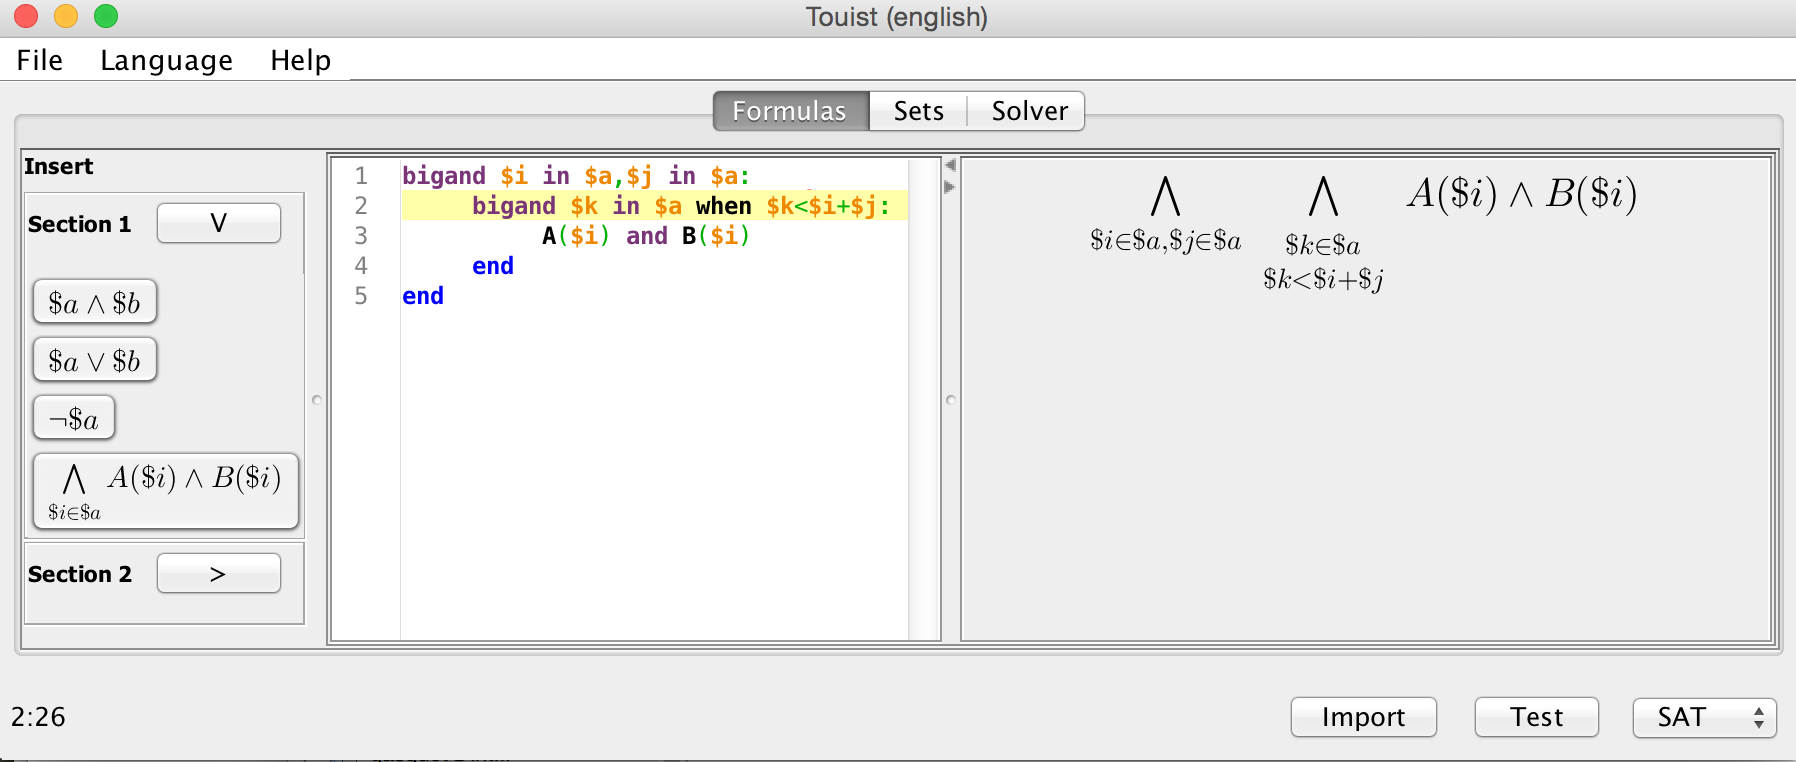
\includegraphics[scale=0.45]{figures/LatexDisplay.png}
  \caption{Affichage en style \LaTeX}
  \label{fig:LatexDisplay}
\end{figure*}


En outre, les formules peuvent être tapées à la main dans la fenêtre d'édition, ou introduites dans une sorte d'éditeur dirigé par la syntaxe, en raffinant progressivement l'arbre syntaxique, ou encore elles peuvent être importées à partir d'un fichier externe.





%\begin{figure*}[ht]
%  \centering
%  \includegraphics[scale=.4]{touist1.png}
%  \caption{Interface de TouIST}
%  \label{fig:touist}
%\end{figure*}


\subsection{Ébauche de traduction de logiques dynamiques}
...
